\documentclass[tikz,border=10pt]{standalone}
\usetikzlibrary{angles}
\begin{document}
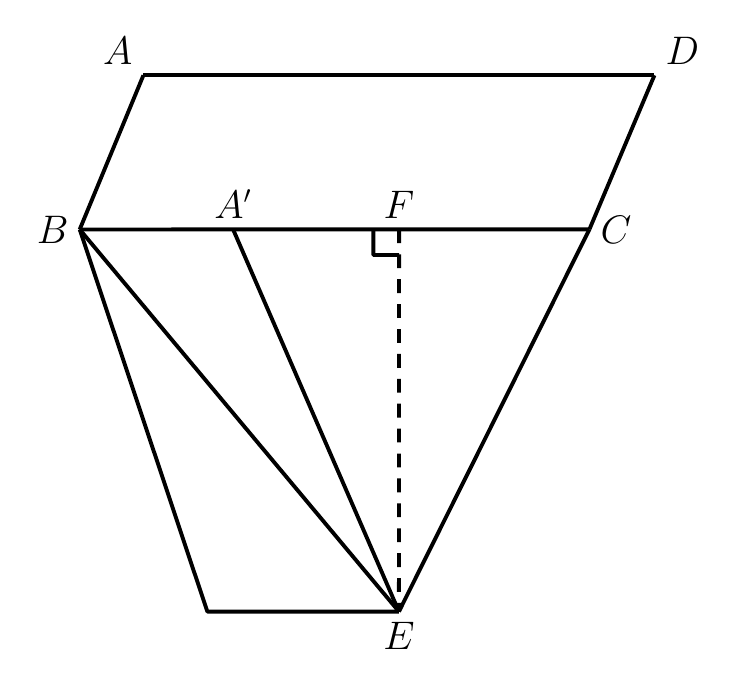
\begin{tikzpicture}[line width=1.4pt, line join=round,
  every node/.style={font=\fontsize{13.5}{16.2}\selectfont}]
\coordinate (A) at (-2.680,3.416);
\coordinate (B) at (-3.489,1.458);
\coordinate (C) at (2.984,1.459);
\coordinate (D) at (3.810,3.416);
\coordinate (F) at (0.567,1.459);




\coordinate (E) at (0.565,-3.395);
\coordinate (Ap) at (-1.541,1.459);
\coordinate (J) at (-1.868,-3.395);


\draw (A) -- (D);
\draw (A) -- (B);
\draw (C) -- (D);
\draw (B) -- (F) -- (C);
\draw (B) -- (J) -- (E);
\draw (B) -- (E);
\draw (C) -- (E);
\draw (Ap) -- (E);
\draw[dashed, dash pattern=on 5pt off 4pt] (F) -- (E);


\draw pic[draw, angle radius=0.326cm] {right angle=B--F--E};


\node[above left] at (A) {$A$};
\node[above right] at (D) {$D$};
\node[left] at (B) {$B$};
\node[right] at (C) {$C$};
\node[above] at (F) {$F$};
\node[below] at (E) {$E$};
\node[above] at (Ap) {$A'$};
\end{tikzpicture}
\end{document}